\documentclass[border=10pt]{standalone}
\usepackage{pgfplots}
\pgfplotsset{compat=1.18}

\begin{document}
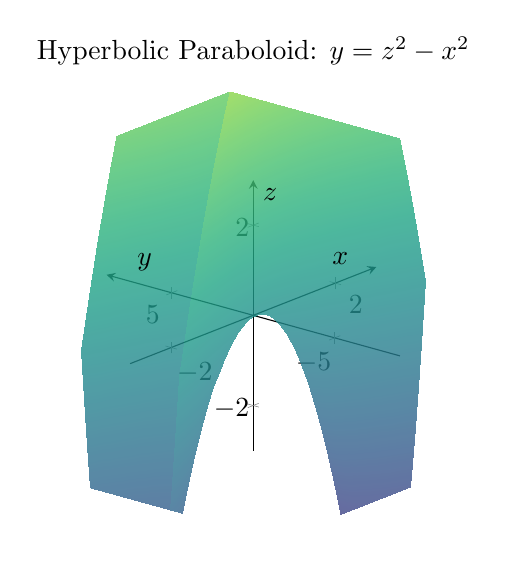
\begin{tikzpicture}
\begin{axis}[
    xlabel=$x$,
    ylabel=$y$,
    zlabel=$z$,
    title={Hyperbolic Paraboloid: $y = z^2 - x^2$},
    view={-50}{25},
    colormap/viridis,
    grid=none,
    axis lines=center,
    domain=-3:3,
    y domain=-3:3,
    samples=50,
    samples y=50,
    zmin=-3, zmax=3,
    xmin=-3, xmax=3,
    ymin=-9, ymax=9,
]
\addplot3[surf, opacity=0.8, shader=interp] {y^2 - x^2};
\end{axis}
\end{tikzpicture}
\end{document}